\documentclass[a4paper,11pt]{article}

\usepackage[utf8]{inputenc}
\usepackage[T1]{fontenc}
\usepackage[french]{babel}
% \usepackage{fullpage}
\usepackage{amsmath, amsfonts, amssymb, amsthm}
% \usepackage{mathabx}
% \usepackage{bbm}
\usepackage{stmaryrd}
\usepackage{graphicx}
% \usepackage{enumerate}

% notations textuelles condensées
	\newcommand{\ssi}{si, et seulement si, }
	\newcommand{\ps}{\ensuremath{\text{ p.s.}}}



% restriction d'applications
	\newcommand{\restrictionaux}[2]{{#1\,\smash{\vrule height .8\ht1 depth .85\dp1}}_{\,#2}}
	\newcommand{\restr}[2]{\ensuremath{\mathchoice
		{\setbox1\hbox{${\displaystyle #1}_{\scriptstyle #2}$}
		\restrictionaux{#1}{#2}}
		{\setbox1\hbox{${\textstyle #1}_{\scriptstyle #2}$}
		\restrictionaux{#1}{#2}}
		{\setbox1\hbox{${\scriptstyle #1}_{\scriptscriptstyle #2}$}
		\restrictionaux{#1}{#2}}
		{\setbox1\hbox{${\scriptscriptstyle #1}_{\scriptscriptstyle #2}$}
		\restrictionaux{#1}{#2}}}}



% notations mathématiques
	% applications
		\newcommand{\map}[4]{\ensuremath{\begin{array}{r c l}#1&\to&#2\\#3&\mapsto&#4\end{array}}}
		\newcommand{\mapp}[6]{\ensuremath{\begin{array}{r c l}#1&\to&#2\\#3&\mapsto&#4\\#5&\mapsto&#6\end{array}}}

	% listes d'éléments
		\newcommand{\set}[1]{\ensuremath{\left\lbrace #1 \right\rbrace}}
		\newcommand{\scal}[2]{\ensuremath{\left<#1,#2\right>}}
		\newcommand{\couple}[2]{\ensuremath{\left(#1,#2\right)}}
		\newcommand{\seq}[2]{\ensuremath{\displaystyle{\left(#1\right)_{#2}}}}

	% notations d'Euler
		\newcommand{\integrale}[2]{\ensuremath{\displaystyle{\int_{#1}^{#2}}}}
		\newcommand{\somme}[2]{\ensuremath{\displaystyle{\sum_{#1}^{#2}}}}
		\newcommand{\produit}[2]{\ensuremath{\displaystyle{\prod_{#1}^{#2}}}}
		\newcommand{\union}[2]{\ensuremath{\displaystyle{\bigcup_{#1}^{#2}}}}
		\newcommand{\inter}[2]{\ensuremath{\displaystyle{\bigcap_{#1}^{#2}}}}
		\newcommand{\sommedirecte}[2]{\ensuremath{\displaystyle{\bigoplus_{#1}^{#2}}}}
		\newcommand{\tensoriel}[2]{\ensuremath{\displaystyle{\bigotimes_{#1}^{#2}}}}
		\newcommand{\cartesien}[2]{\ensuremath{\displaystyle{\bigtimes_{#1}^{#2}}}}

	% normes
		\newcommand{\abs}[1]{\ensuremath{\left| #1 \right|}}
		\newcommand{\norm}[1]{\ensuremath{\left\| #1 \right\|}}

	% probabilités
		\newcommand{\univers}{\ensuremath{\left(\Omega, \mathcal F, \mathbb P \right)}}
		\newcommand{\proba}[1]{\ensuremath{\mathbb P\left(#1\right)}}



% mise en forme
	\newcommand{\notion}{}



% préférences personnelles de typographie
	\renewcommand{\epsilon}{\varepsilon}
	% \renewcommand{\phi}{\varphi}
	\renewcommand{\tilde}{\widetilde}
	\renewcommand{\hat}{\widehat}
	\renewcommand{\bar}{\widebar}



% opérateurs mathématiques
	\DeclareMathOperator{\id}{id}
	\DeclareMathOperator{\Ran}{Im}
	\DeclareMathOperator{\Ker}{Ker}
	\DeclareMathOperator{\Tr}{Tr}
	\DeclareMathOperator{\supp}{supp}
	\DeclareMathOperator{\Vect}{Vect}
	\DeclareMathOperator{\pr}{pr}
	\DeclareMathOperator{\Int}{Int}
	%\DeclareMathOperator{\ln}{ln}



% théorèmes
	\theoremstyle{plain} %résultats
		\newtheorem{thm}{Théorème}[section]
		\newtheorem{cor}[thm]{Corollaire}
		\newtheorem{pte}[thm]{Propriété}
		\newtheorem{prop}[thm]{Proposition}
		\newtheorem{res}[thm]{Résultat}
		\newtheorem{lem}[thm]{Lemme}
	\theoremstyle{definition} %définitions
		\newtheorem{definition}[thm]{Définition}
	\theoremstyle{remark} %remarques
		\newtheorem*{rk}{Remarque}

\title{Projet de simulations aléatoires : Modèles d'Ising}
\author{Aurélien Enfroy, Shmuel Rakotonirina{-}-Ricquebourg}

\begin{document}
\maketitle

\section{Implémentation du modèle d'Ising}

On rappelle la définition du modèle d'Ising sur un réseau carré :
\begin{definition}
On fixe $C$ le réseau carré de dimension 2 de taille $N^2$. Le modèle d'Ising est la distribution sur l'espace d'état $\set{\pm 1}^C$ dont la loi est donnée par
$$\forall x \in \set{\pm 1}^C, \pi(x) = \frac{1}{Z_T} \exp \left(\left( \somme{u\sim v}{} J_{u,v} x_{u} x_{v} + \somme{u}{} h_{u} x_{u} \right)/T\right)$$
où $T>0$ est appelée la température, $Z_T$ est une constante de normalisation, $J_{u,v}$ est la force d'interaction entre $u$ et $v$ et $h_{u}$ est le champ magnétique extérieur en $u$.
\end{definition}

Pour l'implémentation, on remarque qu'il n'y a pas besoin du paramètre $T$, qu'on peut compter dans $J$ et $h$. On représente alors ces paramètres en prenant $x \in \mathcal M_{N,N}(\set{\pm 1})$, $h \in \mathcal M_{N,N}(\mathbb R)$ et $J$ comme une matrice à trois entrées $\tilde J \in \mathcal M_{N,N,2}(\mathbb R)$ où
$$\tilde J_{i,j,1} = J_{(i,j),(i+1,j)} \text{ et } \tilde J_{i,j,2} = J_{(i,j),(i,j+1)}$$
où $i+1$ et $j+1$ sont à comprendre modulo $N$ pour obtenir des conditions aux bords périodiques.

\section{Simulation naïve en petite taille}

En petite taille, on peut faire une simulation naïve. Pour cela, on numérote les $2^{N^2}$ états (dans l'ordre lexicographique en lisant les matrices colonne par colonne), on calcule exactement la loi et on choisit un numéro en utilisant cette loi et une loi uniforme sur $[0,1]$.

\section{Simulation par Metropolis-Hastings}\label{sec:MH}

Nous avons implémenté l'algorithme de Metropolis-Hastings en utilisant la fonction de rejet de Metropolis-Hastings. Pour le choix du noyau instrumental $Q$, nous avons choisi de donner à une coordonnée aléatoire (uniforme) une valeur aléatoire (uniforme), ce qui permet d'avoir un noyau symétrique irréductible apériodique (probabilité strictement positive de rester sur place).

Avec ce noyau instrumental, on peut réduire les calculs effectués : si $x$ est un état et $y$ l'état proposé à partir de $x$, alors
\begin{itemize}
	\item soit $y = x$, auquel cas on peut considérer qu'on accepte le mouvement,
	\item soit $y \neq x$, auquel cas ils ne diffèrent que d'au plus une coordonnée (celle tirée uniformément). Si on note $u$ cette coordonnée et $s$ la nouvelle valeur, alors $s = y_u = - x_u$ et, en considérant que $T$ a été pris en compte dans $J$ et $h$,
	\begin{align*}
	\frac{\pi(y)}{\pi(x)}
	&= \frac{\exp \left( \somme{v \sim u}{} J_{u,v} s x_{v} + h_{u} s \right)}{\exp \left( \somme{v \sim u}{} J_{u,v} (-s) x_{v} + h_{u} (-s) \right)}\\
	&= \frac{e^{s V_u(x)}}{e^{-s V_u(x)}}\\
	&= e^{2 s V_u(x)}
	\end{align*}
	où on a noté $V_u(x) \doteq \somme{v \sim u}{} J_{u,v} x_v + h_u$.
\end{itemize}

\section{Simulation par l'échantilloneur de Gibbs}

En reprenant les notations du cours, on a pour $u \in C$ et $x \in \set{\pm 1}^C$, en considérant que $J$ et $h$ dépendent de $T$,
\begin{align*}
\pi_u(x_u \mid x^u)
&= \frac{\pi(x_u,x^u)}{\pi(1,x^u) + \pi(-1,x^u)}\\
&= \frac{e^{x_u V_u(x)}}{e^{V_u(x)} + e^{-V_u(x)}}
\end{align*}
où on note encore $V_u(x) \doteq \somme{v \sim u}{} J_{u,v} x_v + h_u$. Donc $\pi_u(\cdot \mid x^u) = \mathcal B(\frac{e^{V_u(x)}}{e^{V_u(x)} + e^{-V_u(x)}}) = B(\frac{1}{1 + e^{-2V_u(x)}})$

\section{Couplage par le passé}

Pour le couplage par le passé, deux fonctions d'actualisation sont possibles. Celle vue en cours est celle issue de l'échantillonneur de Gibbs (par balayage séquentiel). L'autre, présente dans le livre de Propp-Wilson, est issue de l'algorithme de Metropolis-Hastings (i.e. même transition qu'en section \ref{sec:MH}).

L'algorithme consiste à répéter les algorithmes vers le futur jusqu'à un temps donné et, si il n'y a pas eu coalition, ajouter des nouvelles actualisations au début du processus, ce qui demande de recommencer du début. Pour gagner du temps, plutôt que d'ajouter une actualisation à chaque fois, on double le nombre d'actualisations.

Pour les deux méthodes (Metropolis-Hastings et échantillonneur de Gibbs), les choses se passent bien au-delà de la température critique. Cependant, en dessous de la température critique, les états $\pm(1,\hdots,1)$ ont tendance à rester inchangés par les fonctions d'actualisation précédentes : dans les deux cas, la probabilité de réussir à changer un point $x_u$ égaux à ses quatre voisins est très faible : pour $J/T = \alpha$ constant, $h = 0$, elle vaut $\exp(-8 \alpha)$.

En conséquence, l'algorithme met extrêmement longtemps à terminer (nous n'avons pas vu terminer). En observant l'évolution des chaînes de Markov (parties de $(1,\hdots,1)$ et de $(-1,\hdots,-1)$), on voit que souvent les deux chaînes reviennent à leur état initial, ce qui signifie que tout ce qui a été simulé jusqu'ici a été une perte de temps.

\section{Vérification des algorithmes}

Pour vérifier que les algorithmes MCMC fonctionnent, on vérifie l'ergodicité sur la fonction $M(x) = \frac{1}{N^2} \sum_u x_u$. $M$ est appelée la magnétisation. Dans le cas où $h = 0$, on a $\pi(-x) = \pi(x)$ et $M(-x) = -M(x)$ donc si $X \sim \pi$, alors $\mathbb E(M(X)) = 0$. Si la chaîne $(X^{(n)})_n$ est ergodique, on aura donc la convergence presque sûre
$$\frac{1}{n} \sum_i M(X^{(i)}) \xrightarrow[n \rightarrow +\infty]{} 0$$
En pratique, à basse température, les algorithmes ont tendance à rester longtemps dans les états $(1,\hdots,1)$ et $(-1,\hdots,-1)$ (qui sont très probables à basse température) donc il faudrait attendre un temps très long pour voir cette convergence. On se place donc à haute température.

Pour l'algorithme exact (couplage par le passé), on simule de manière indépendante un échantillon $(X^{(n)})_n$ et on vérifie que la loi des grands nombres s'applique :
$$\frac{1}{n} \sum_i M(X^{(i)}) \xrightarrow[n \rightarrow +\infty]{} 0.$$

On obtient les résultats de la figure \ref{fig:ergodic}.
\begin{figure}
	\label{fig:ergodic}
	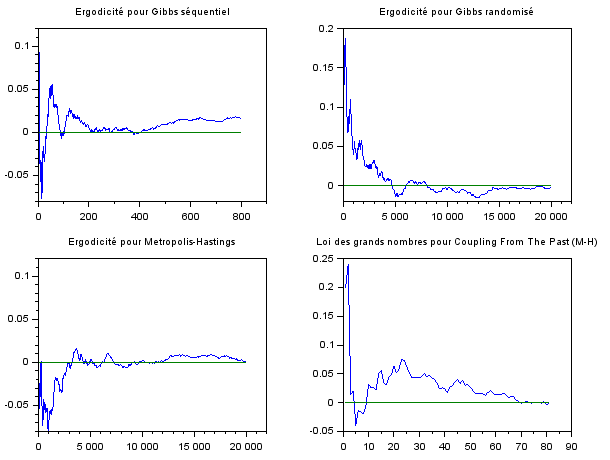
\includegraphics[width=0.8\textwidth]{ergodicite_magnetisation.png}
	\caption{Vérification de l'ergodicité et de la loi des grands nombres sur la magnétisation}
\end{figure}

\end{document}